\section{JTAG}
Scansta112 is 7-Port Multidrop JTAG Multiplexer. It is used to partition scan chains into managable sizes, or to isolate specific devices onto a separate chain. By default Scansta input signal is from IDC header. AMC JTAG is connected to Master Port on SCANSTA, so it can be used as Master or Slave module. The rest modules (MMC, FPGA, FMC, RTM) are tied to slave SCANSTA outputs. \\

Tere are two JTAG sources – either AMC connector ( JSM module) or USB to JTAG bridge (FTDI chip). There is also onboard JTAG connector (Xilinx type) -J3. Insertion of JTAG programmer probe deactivates the FTDI JTAG connectivity and forces SCANSTA chip set this port as master port. By default SCANSTA selects AMC port as master one.\\


In Sayma AMC, SCANSTA112 is used in Transparent Sticher Mode. In this mode, the IC can be configured via hardware to skip the addressing protocol needed, sothere is no need to run a SVF configuration file on IMPACT when programming the FPGA bitstream.\\
	\begin{figure}[htbp!]
		\centering
		\includegraphics[scale=0.5]{img/jtag.png}\\
		\caption{USB-->JTAG} 
	\end{figure}
\clearpage	
General block scheme of Scansta connections is shown below.\\
	
		\begin{figure}[htbp!]
			\centering
			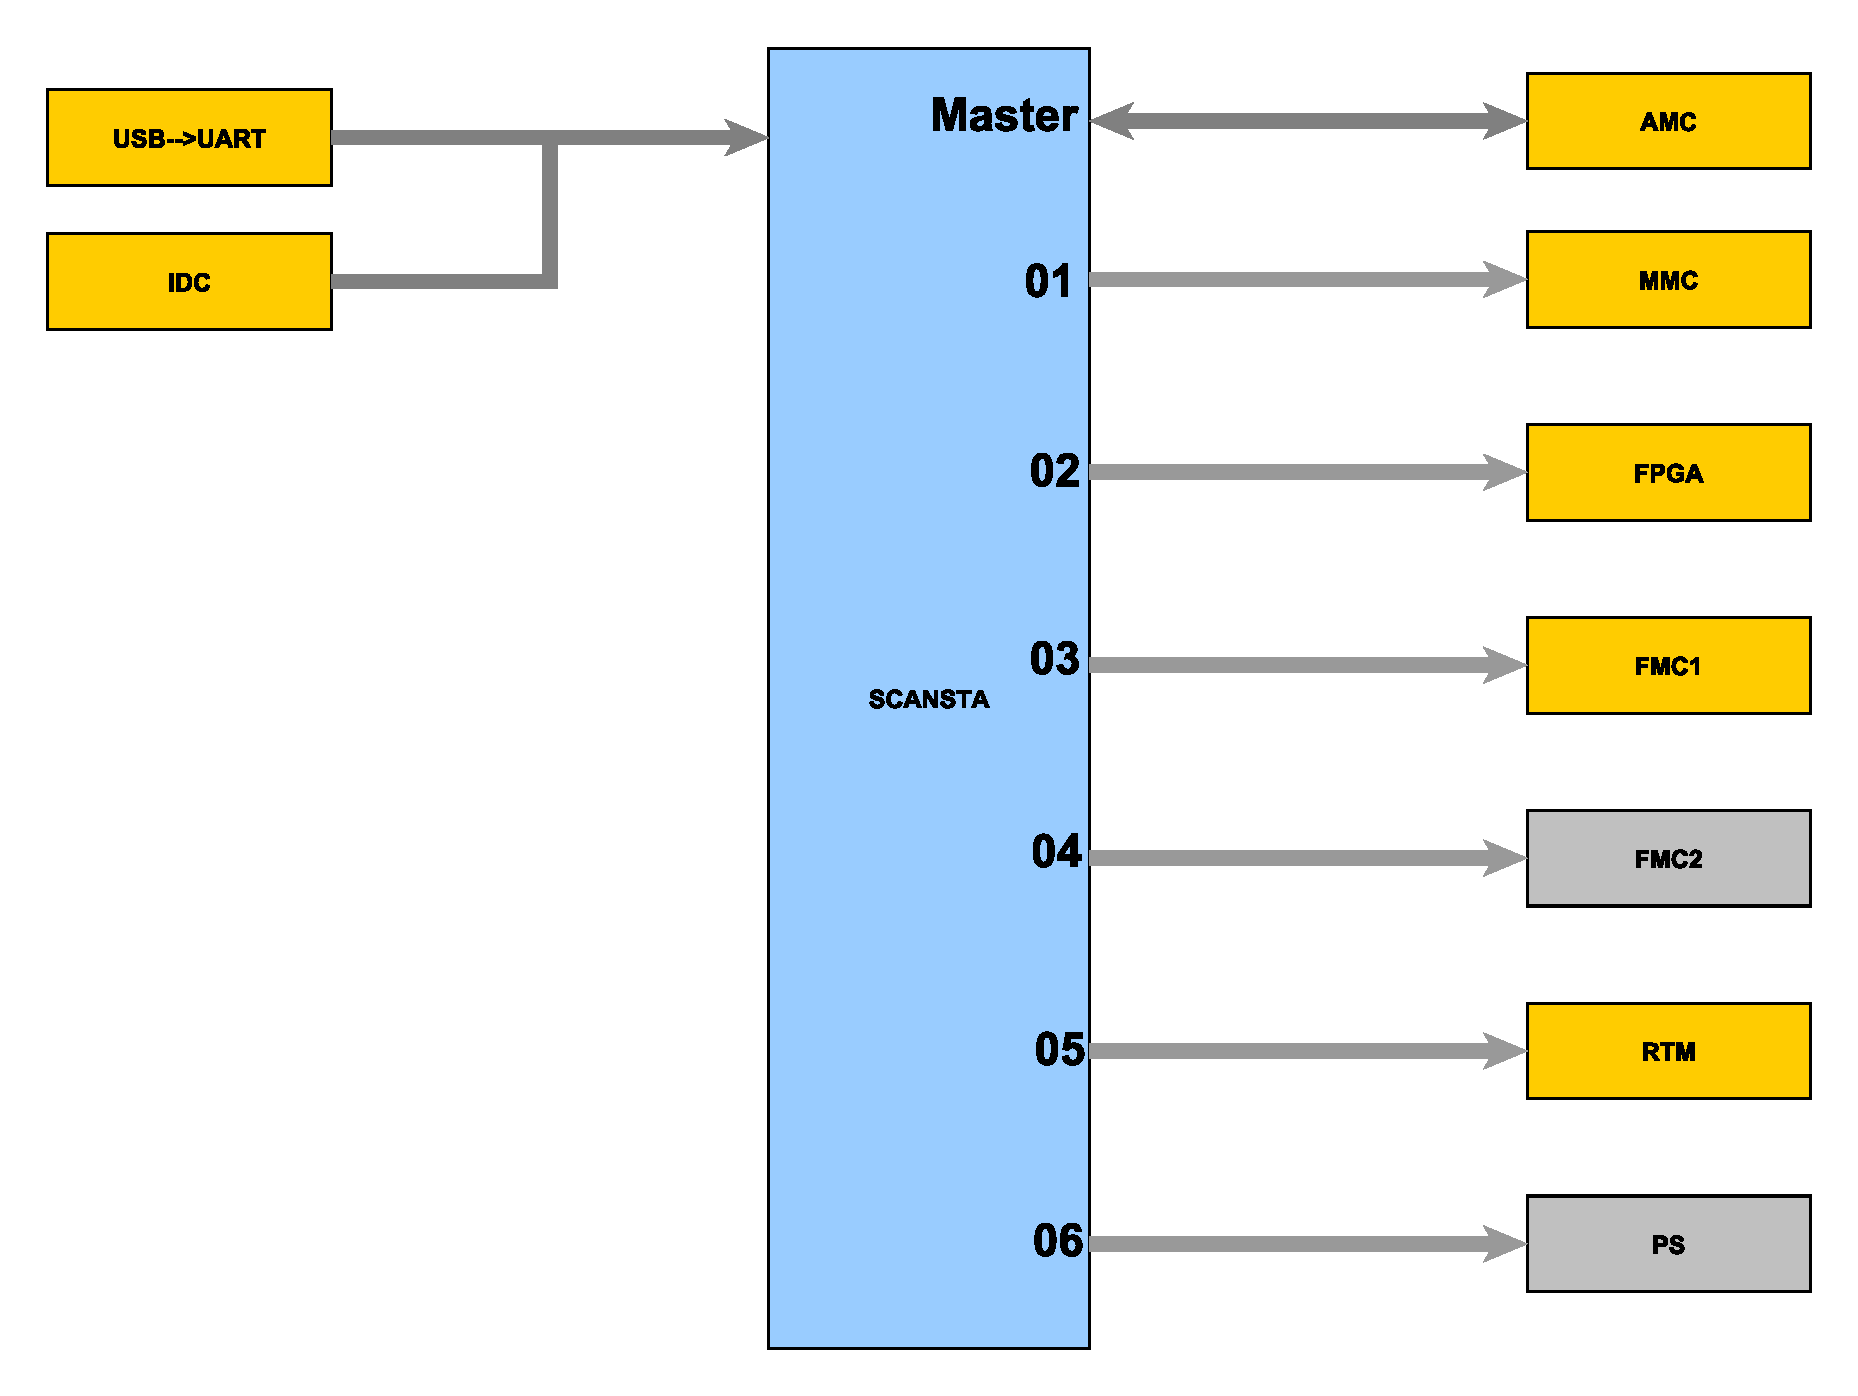
\includegraphics[scale=0.4]{img/scansta.eps}\\
			\caption{SCANSTA bloch scheme} 
		\end{figure}
		
	\textit{\textbf{Note:} The FMC2 and PS is not used.}\\


Each of JTAG slave devices is connected directly to SCANSTA. SCANSTA allows to connect all devices in chain witn an option to pass one or more devices, intention in Figure \ref{jtagchain}.

		\begin{figure}[htbp!]
			\centering
			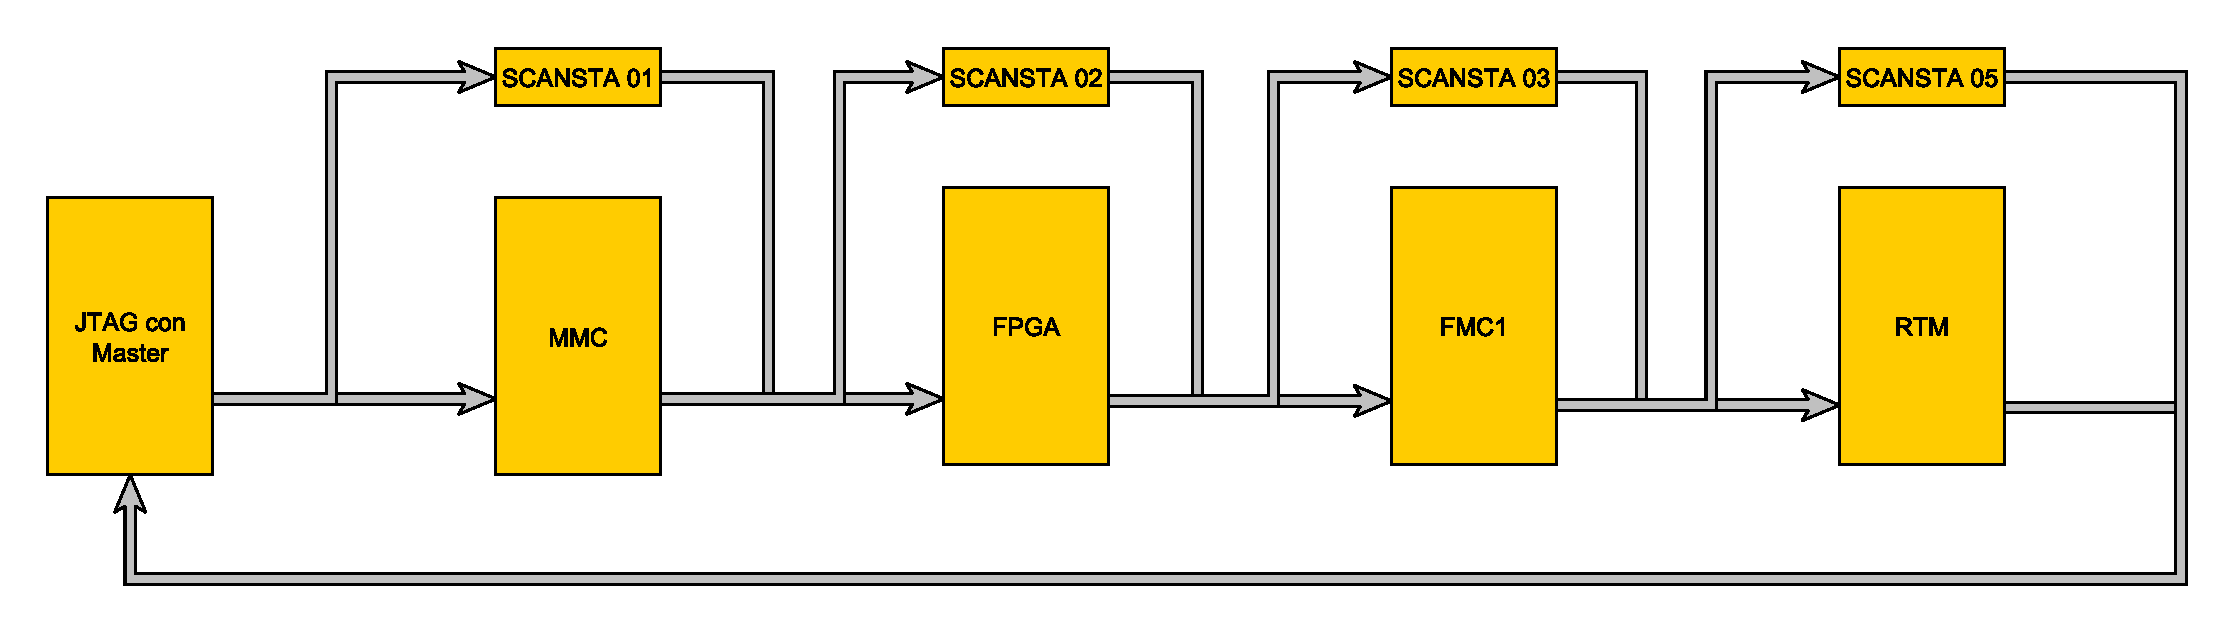
\includegraphics[scale=0.4]{img/jtagchain.eps}\\
			\caption{SCANSTA JTAG chain} \label{jtagchain}
		\end{figure}
		
		
Simplified instruction if using SCANSTA can be found under: \href{http://www.ti.com/lit/an/snla068c/snla068c.pdf}{http://www.ti.com/lit/an/snla068c/snla068c.pdf} 
